%\documentclass[twocolumn,amsmath,amssymb]{report}
\documentclass[twocolumn,amsmath,amssymb]{snp}
\pagestyle{empty}
\usepackage{graphicx}% Include figure files
\usepackage{dcolumn}% Align table columns on decimal point
\usepackage{bm}% bold math
\topmargin 1.5 cm
\textwidth14.5cm
\textheight20cm
\oddsidemargin0.7cm
\columnsep0.2in
\begin{document}

\title{{\Large Study of ``QGSP\_BIC\_HP" and ``QGSP\_BERT\_HP" physics models to simulate neutron transport and transmutation by adiabetic resonance crossing in accelerator driven system }}% Force line breaks with \\

\author{\large Abhijit Bhattacharyya}
\email{vega@barc.gov.in, abhihere@gmail.com}

% \altaffiliation[Also at ]{Physics Department, XYZ University.}%Lines break automatically or can be forced with \\
\affiliation{Nuclear Physics Division, Bhabha Atomic Research Centre, Mumbai - 400085, INDIA}

\maketitle


\section*{Introduction}
Transmutation by Adiabetic Resonance Crossing ($TARC$) \cite {ps211, tarcNIM} concept was first conceived by Carlo Rubbia at CERN-PS facility to test physics concepts related to the radioactive waste management and due to concurrent fission process estimation of energy gained in Energy Amplifier. The Energy Amplifier ($EA$) \cite {ps211, tarcNIM} is a fast neutron subcritical system driven where high energy proton from a proton accelerator is bombarded on a spallation target. For subsequent reactions, EA also contains neutron moderator, heat extraction agent and neutron confinement medium. Beside this, TARC facility may also generate radio-active elements for medical treatment through neutron capture on stable elements.

Natural lead is usually used as spallation target as it shows transparency to neutrons, possessing high and energy independent elastic scattering cross section, moderate slowing down effect owing to small lethargic steps and nearly isotropic elastic scattering helping long neutron storage \cite {ps211, tarcNIM}.

The present paper discusses simulation of neutronics for TARC comparing Geant4 physics models and also comparing with TARC experimental data establishing the reliability of this code. 

\section*{Development of simulation tools}
The simulation was performed using \textsl{Geant4 - $10.5.0$-{\it{beta}} - multithreading mode} - a toolkit written in \textit{C++}. The results were compared for two physics lists namely (\textit{QGSP Binary Cascade Model $<\sim 10 GeV$}) and (\textit{QGSP Bertini Cascade model $< \sim 10 GeV$}) both coupled to \textit{High Precision Model for neutrons} ($HP$ $<20 MeV$). Here \textit{QGSP} stands for Quark Gluon String Physics model.

While the paper compares results with two physics models as stated, simulation results are compared with TARC experimental data to check the reliability of the code. For this purpose, 2.5 GeV/c protons were used for spallation. The Geometry used in this simulation was taken from TARC group as $GDML$ file. This ensures possibility of transferring any geometry for test from CAD drawing to GDML directly. 


\section*{Figures and Tables}
<<<<<<< HEAD
Here, few results are presented.

\begin{figure*}
    \centering 
=======
Few results are presented here.

\begin{figure*}
    \centering 
        \textbf{Comparison of Neutron Energy deposition}\par\medskip
>>>>>>>  code is running in MT
    \begin{minipage}[b]{0.4\textwidth}
    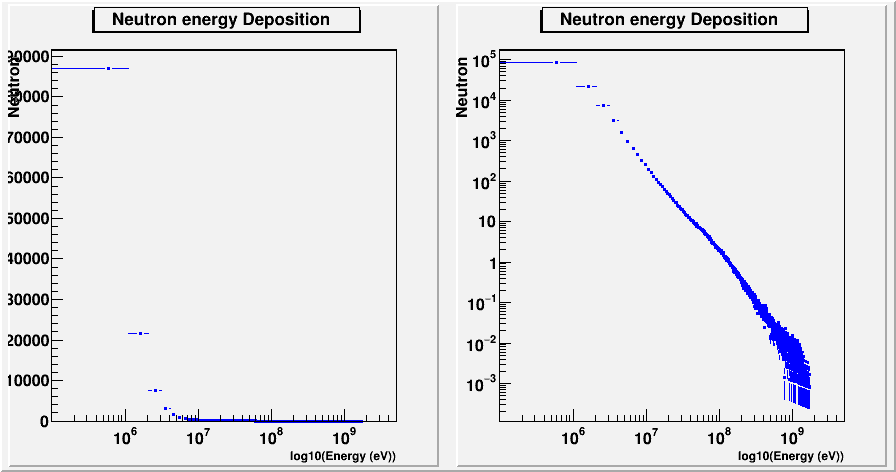
\includegraphics [height=30mm, width=55 mm] {NeutEdepBIC.png}
    \caption{\small Neutron Energy Deposition : QGSP\_BIC\_HP}
    \end{minipage}
    \begin{minipage}[b]{0.4\textwidth}
    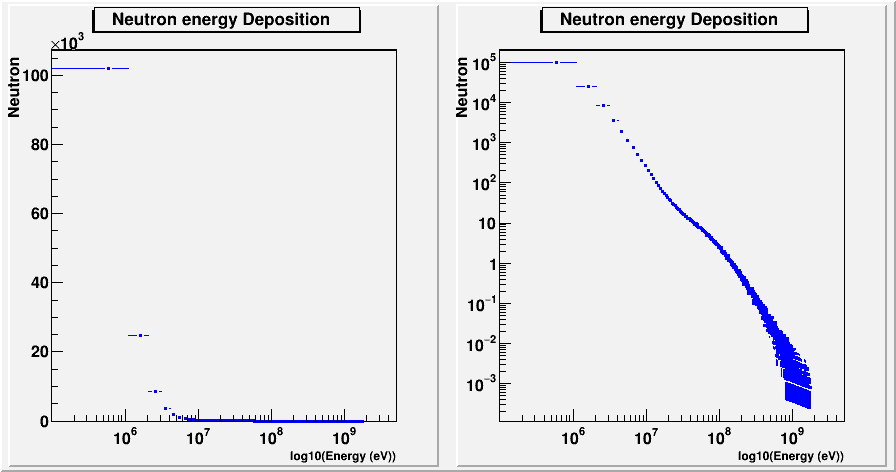
\includegraphics [height=30mm, width=55mm] {NeutEdepBERT.png}
    \caption{\small Neutron Energy Deposition : QGSP\_BERT\_HP}
   \end{minipage}
\end{figure*}


\begin{figure*}
    \centering 
<<<<<<< HEAD
=======
    \textbf{Comparison of correlation between Neutron Energy and time}\par\medskip
>>>>>>>  code is running in MT
    \begin{minipage}[b]{0.4\textwidth}
    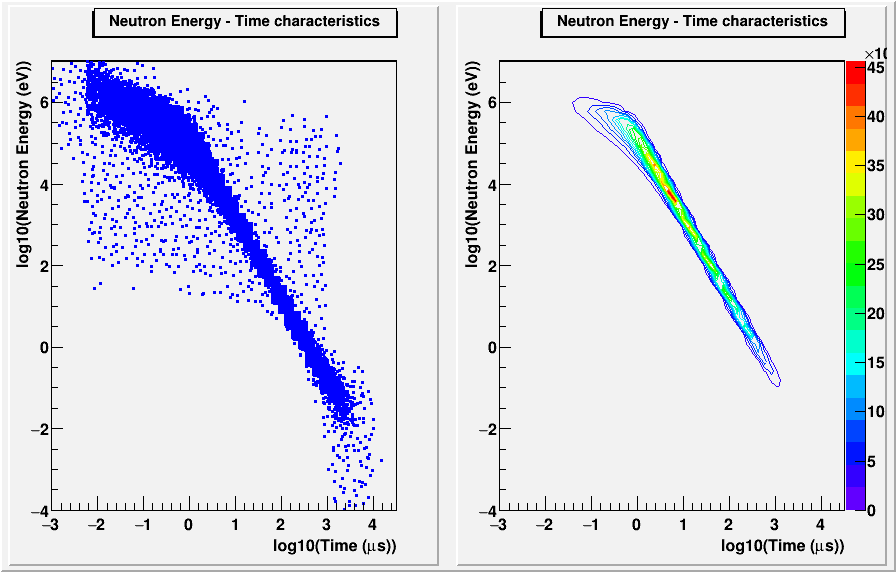
\includegraphics [height=30mm, width=55 mm] {NeutEnergyTimeBIC.png}
    \caption{\small Correlation of Neutron Energy - Time : QGSP\_BIC\_HP}
    \end{minipage}
    \begin{minipage}[b]{0.4\textwidth}
    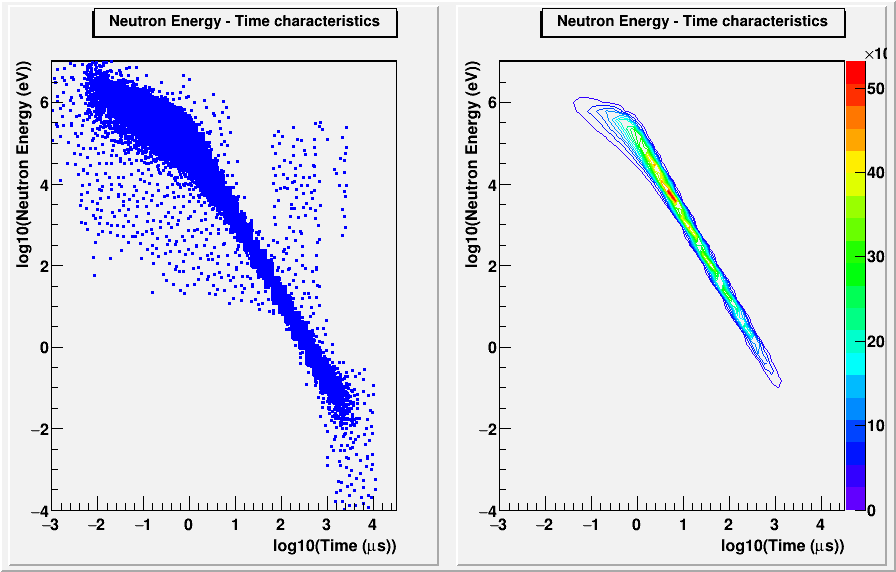
\includegraphics [height=30mm, width=55mm] {NeutEnergyTimeBERT.png}
    \caption{\small Correlation of Neutron Energy - Time : QGSP\_BERT\_HP}
    \end{minipage}
\end{figure*}    


\begin{figure*}
     \centering 
<<<<<<< HEAD
=======
     \textbf{Comparison of correlation between Energy and time for particles other than neutrons}\par\medskip
>>>>>>>  code is running in MT
    \begin{minipage}[b]{0.4\textwidth}
    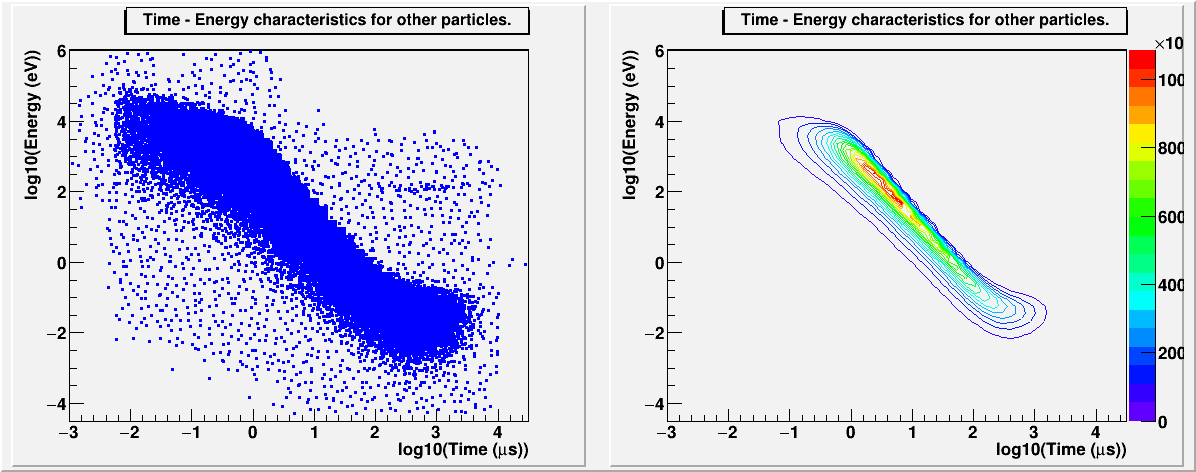
\includegraphics [height=30mm, width=55 mm] {OtherEnergyTimeBIC.png}
    \caption{\small Correlation of Other particles Energy - Time : QGSP\_BIC\_HP}
    \end{minipage}
    \begin{minipage}[b]{0.4\textwidth}
    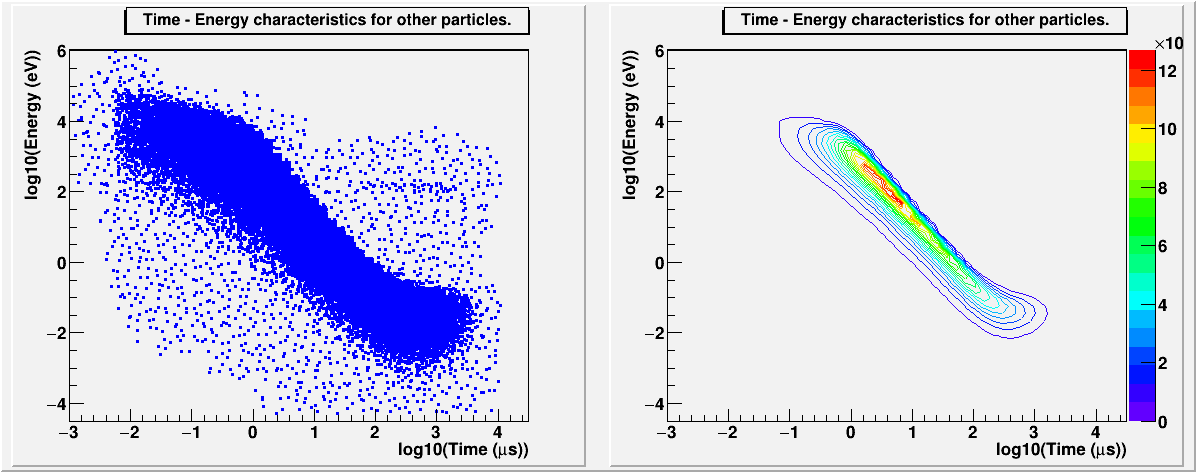
\includegraphics [height=30mm, width=55mm] {OtherEnergyTimeBERT.png}
    \caption{\small Correlation of Other particles Energy - Time : QGSP\_BERT\_HP}
    \end{minipage}
\end{figure*}

\begin{figure*}
    \centering 
<<<<<<< HEAD
=======
    \textbf{Comparison of distribution of fluence against energy}\par\medskip
>>>>>>>  code is running in MT
    \begin{minipage}[b]{0.4\textwidth}
        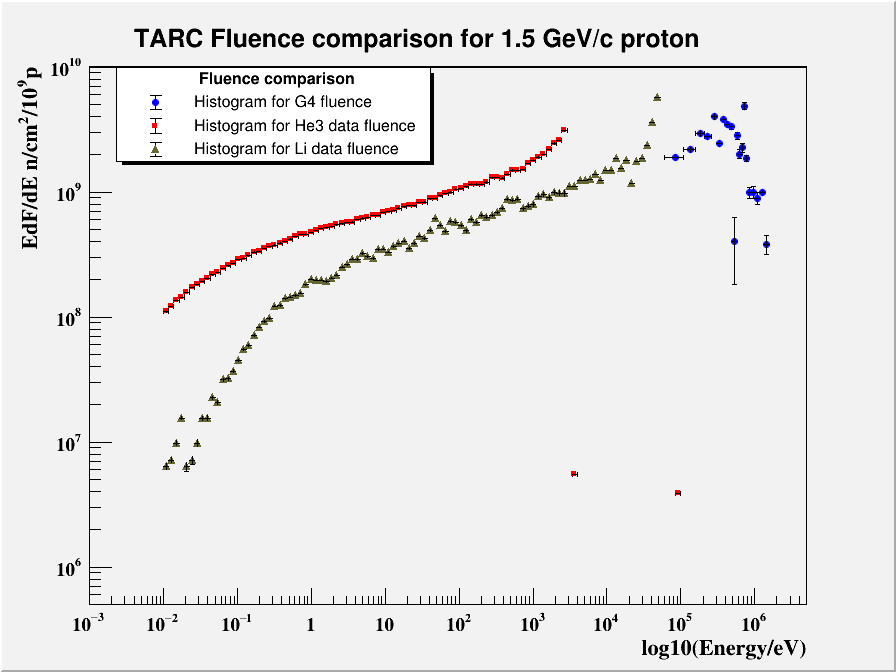
\includegraphics [height=30mm, width=55 mm] {FluenceEnergyBIC.png}
        \caption{\small Distribution of Fluence with Energy : QGSP\_BIC\_HP}
    \end{minipage}
    \begin{minipage}[b]{0.4\textwidth}
        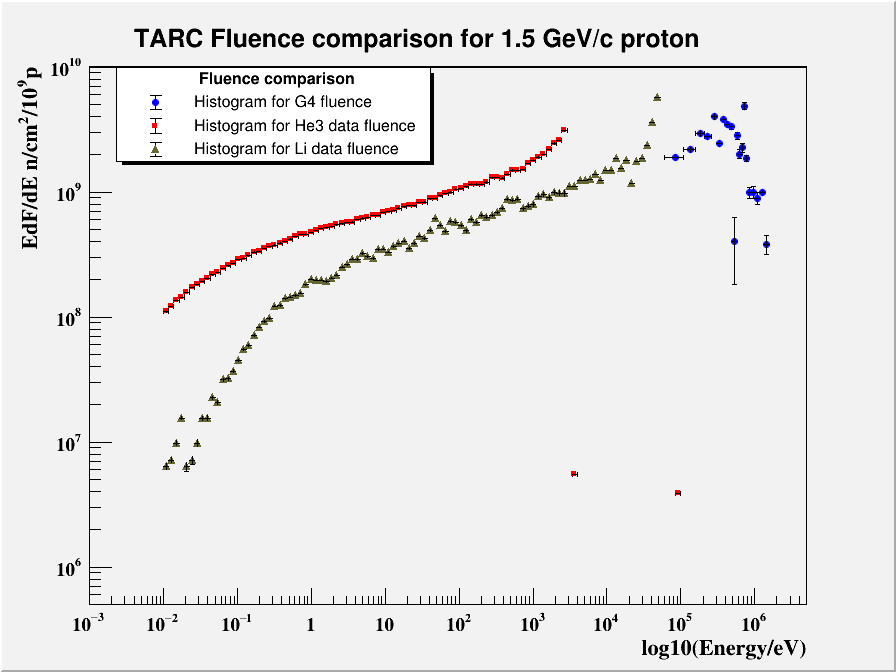
\includegraphics [height=30mm, width=55mm] {FluenceEnergyBERT.png}
        \caption{\small Distribution of Fluence with Energy : QGSP\_BERT\_HP}
    \end{minipage}
\end{figure*}

\begin{figure*}
    \centering 
<<<<<<< HEAD
=======
    \textbf{Comparison of simulation with experimental for two different physics models}\par\medskip
>>>>>>>  code is running in MT
    \begin{minipage}[b]{0.4\textwidth}
        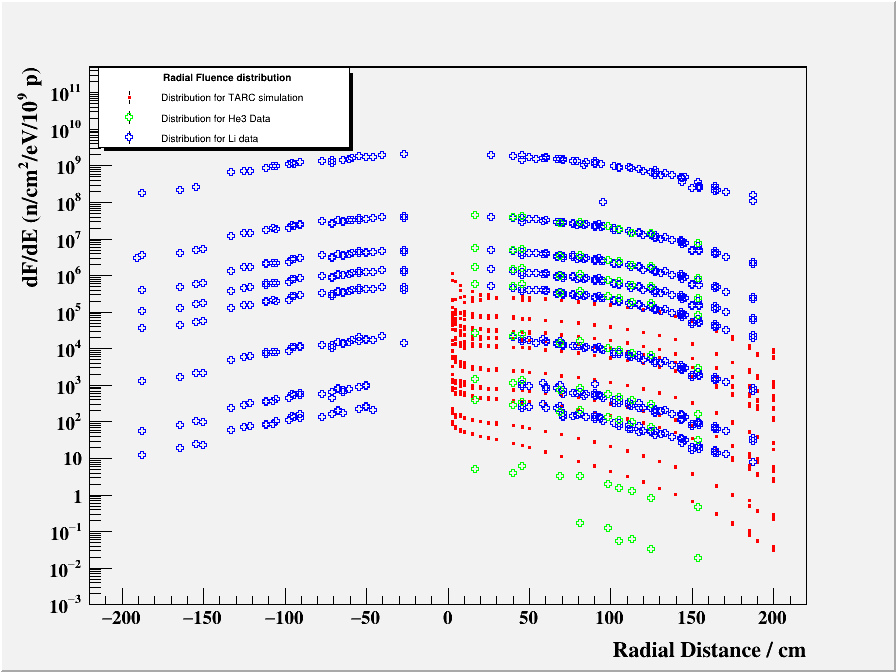
\includegraphics [height=30mm, width=55 mm] {FluenceRadialDistBIC.png}
        \caption{\small Distribution of Fluence with Radial distance : QGSP\_BIC\_HP}
    \end{minipage}
    \begin{minipage}[b]{0.4\textwidth}
        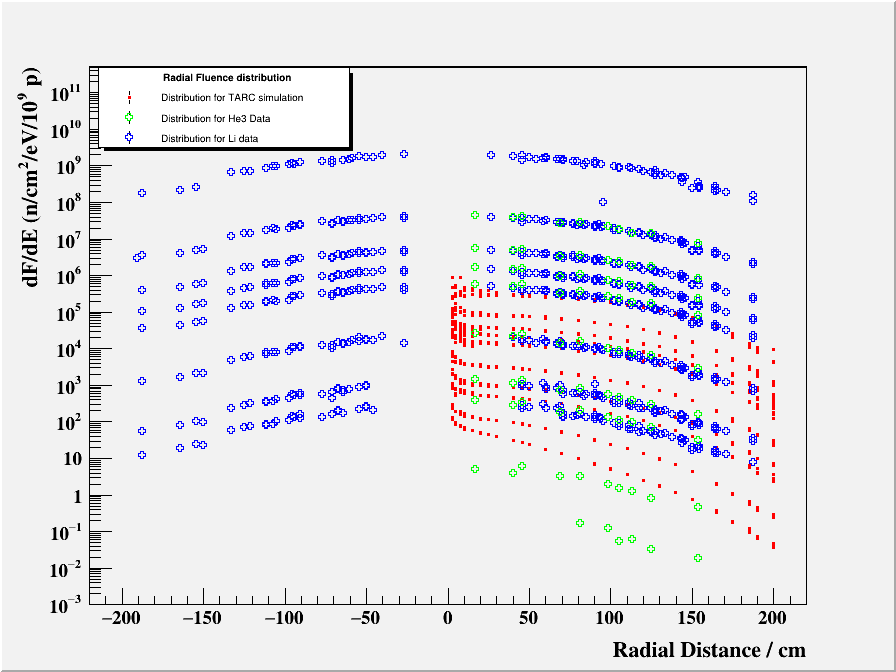
\includegraphics [height=30mm, width=55mm] {FluenceRadialDistBERT.png}
        \caption{\small Distribution of Fluence with Radial distance : QGSP\_BERT\_HP}
    \end{minipage}
\end{figure*}

%\begin{figure*}
%    \centering 
%    \begin{minipage}[b]{0.4\textwidth}
%        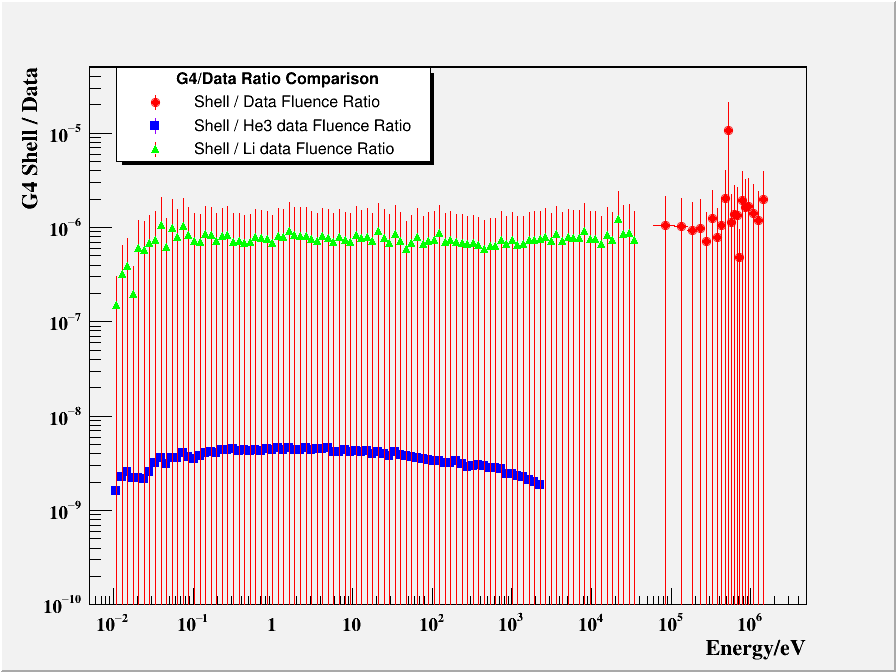
\includegraphics [height=30mm, width=55 mm] {RatioBIC.png}
%        \caption{\small Ratio plot of Fluence G4 with data : QGSP\_BIC\_HP}
%    \end{minipage}
%    \begin{minipage}[b]{0.4\textwidth}
%        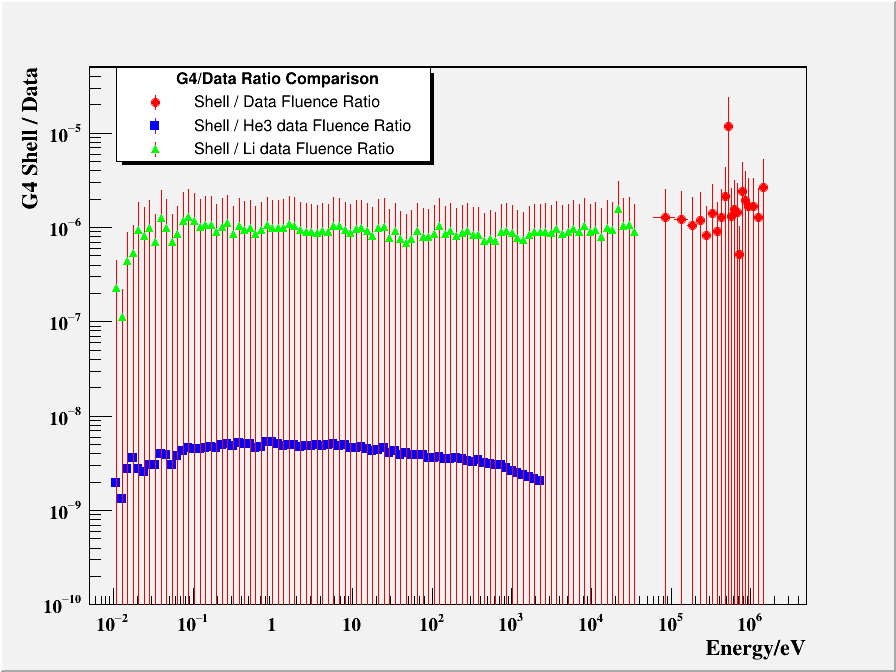
\includegraphics [height=30mm, width=55mm] {RatioBERT.png}
%        \caption{\small Ratio plot of Fluence G4 with data : QGSP\_BERT\_HP}
%    \end{minipage}
%\end{figure*}


\begin{figure*}
    \centering 
<<<<<<< HEAD
=======
    \textbf{Comparison of neutron flux distribution of generated neutron flux }\par\medskip
>>>>>>>  code is running in MT
    \begin{minipage}[b]{0.4\textwidth}
        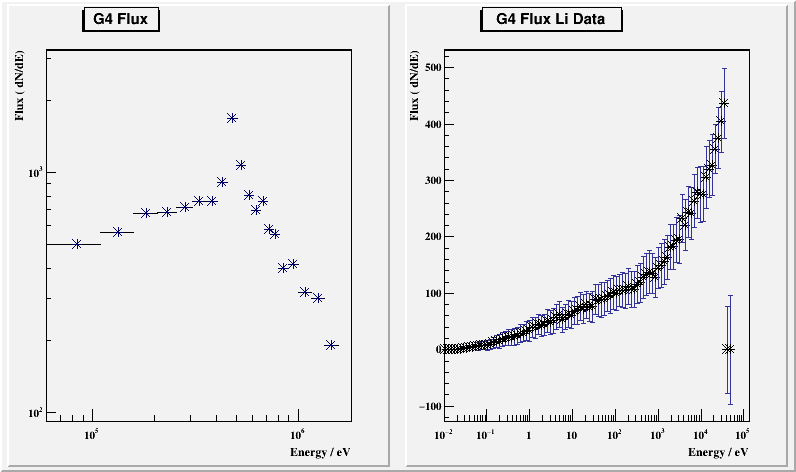
\includegraphics [height=30mm, width=55 mm] {FluxBIC.png}
        \caption{\small Distribution of Flux : QGSP\_BIC\_HP}
    \end{minipage}
    \begin{minipage}[b]{0.4\textwidth}
        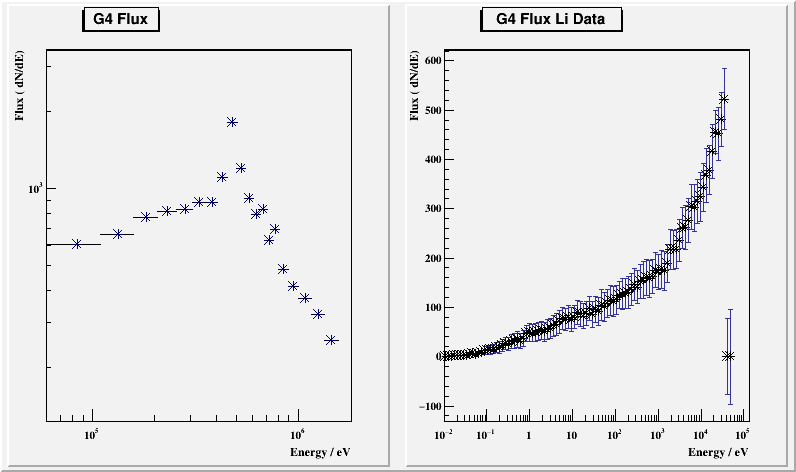
\includegraphics [height=30mm, width=55mm] {FluxBERT.png}
        \caption{\small Distribution of Flux : QGSP\_BERT\_HP}
    \end{minipage}
\end{figure*}



\begin{figure*}
    \centering 
<<<<<<< HEAD
=======
    \textbf{Comparison of spectra of neutrons exited from the system}\par\medskip
>>>>>>>  code is running in MT
    \begin{minipage}[b]{0.4\textwidth}
        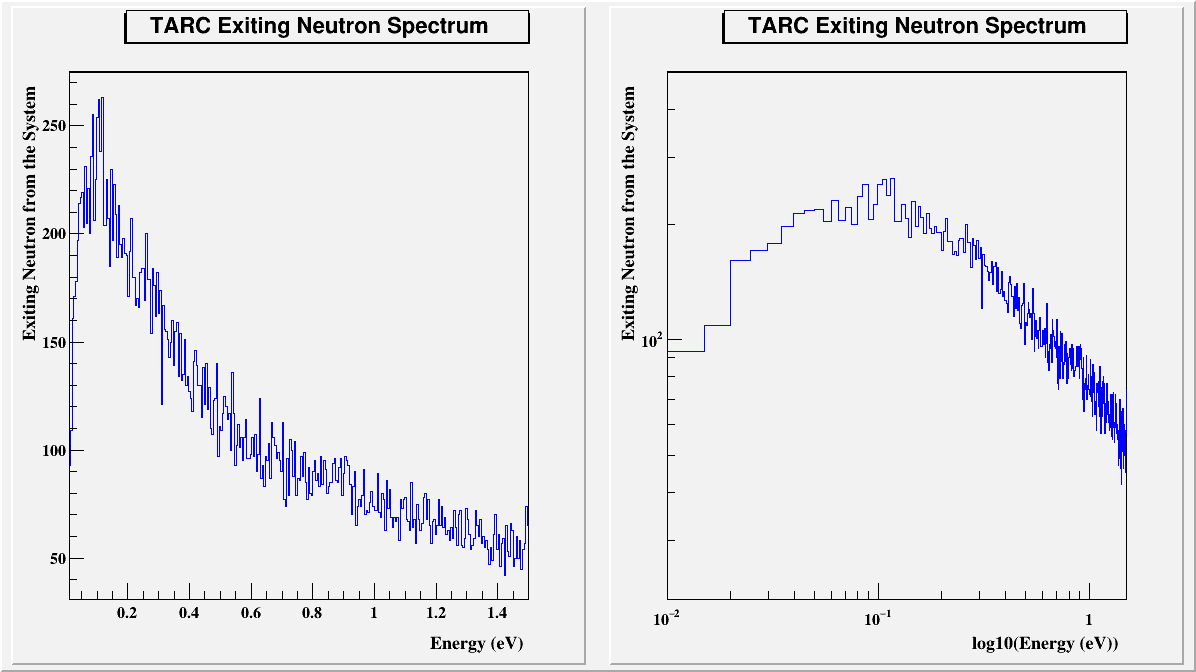
\includegraphics [height=30mm, width=55 mm] {ExitingNSpectrumBIC.png}
        \caption{\small Spectrum of neutrons exiting from the system : QGSP\_BIC\_HP}
    \end{minipage}
    \begin{minipage}[b]{0.4\textwidth}
        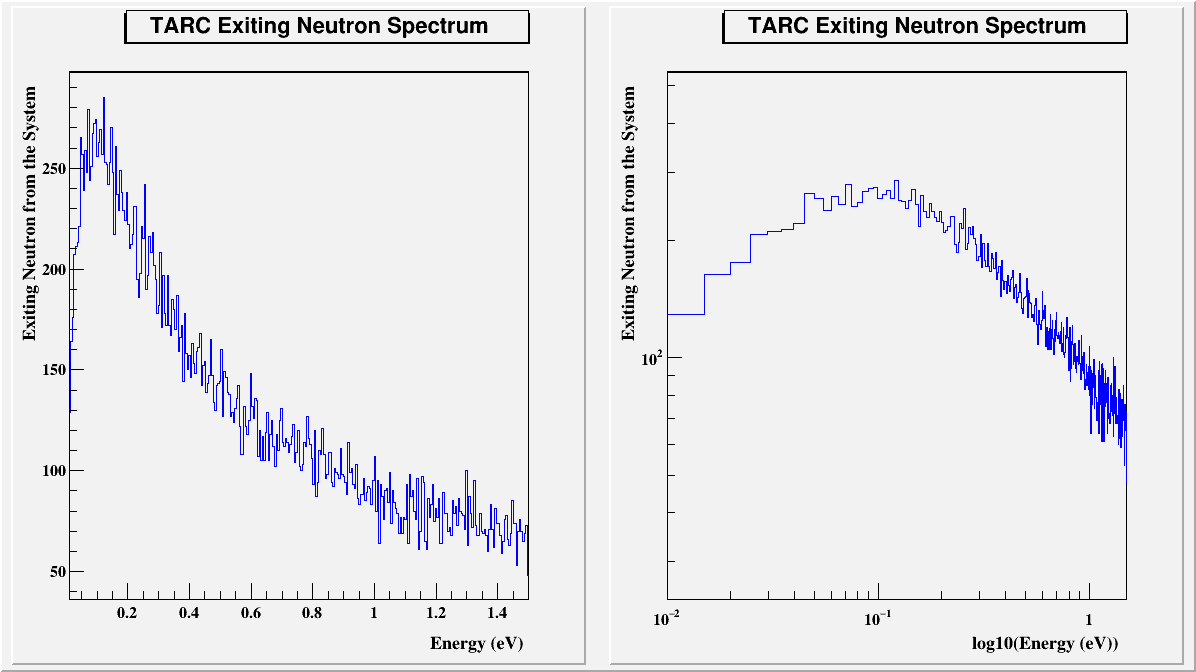
\includegraphics [height=30mm, width=55mm] {ExitingNSpectrumBERT.png}
        \caption{\small Spectrum of neutrons exiting from the system : QGSP\_BERT\_HP}
    \end{minipage}
\end{figure*}


\section*{Acknowledgments}
%\acknowledgments
<<<<<<< HEAD
I thank Alok Saxena, former Head, NPD and Basant K Nayak, NPD, BARC for allowing to work at CERN as Scientific Associate on this simulation modeling. I also thank Federico Carminati,CERN, Alberto Ribon, CERN and Alexander Howard, CERN for useful discussions on different aspects of physics models used in Geant4.
=======
I thank Alok Saxena, former Head, NPD, Basant K Nayak, NPD, BARC, A K Mohanty, Head, NPD \& Director, Physics Group and Vivek Datar, TIFR for my visit to CERN as Scientific Associate on this simulation modeling. I also thank Federico Carminati,CERN, Alberto Ribon, CERN and Alexander Howard, CERN for useful discussions on different aspects of physics models used in Geant4.
>>>>>>>  code is running in MT
%\end{acknowledgments}

%\ \\
%\noindent
\begin{thebibliography}{50}
\bibitem{ps211} The TARC Experiment (PS-211) report, CERN-99-11, Dec 15(1999)
\bibitem{tarcNIM} Results from the TARC experiment, NIM A, {\bf 478}, 577(2002)
%\bibitem{poster} Announcement Poster and Website, DAE Symp. {\bf vv}, ppp (yyyy).
%\bibitem{dae} DAE Symp. on Nucl. Phys. {\bf vv}, ppp (yyyy).
\end{thebibliography}

\end{document}
%
% ****** End of file snpcontrisamp.tex ******
